\section{Histograms of Oriented Gradients}

\begin{frame}{Histograms of Oriented Gradients}
  \metroset{block=fill}
\center
\only<1>{
  \begin{alertblock}{\textbf{Why?}}
  One of the most well known methods for feature extraction for human detection in
  computer vision, it is very versatile and it can be applied in different contexts.
  Ofter it is used as metrix to compare more sophisticated methods.
  \end{alertblock}
}

\only<2>{
  \begin{exampleblock}{\textbf{Idea?}}
  Describe the local behaviour of the gradient applied to an image, in ordet to
  emphasize well defined geometric structures and edges. A local object appearance
  and shape can be characterized by the distribution of local intensity gradients or
  edge directions, even without knowledge of the corresponding gradient.
\end{exampleblock}

}

\only<3>{

\begin{exampleblock}{\textbf{How?}}
  Divide the image window into small spatial regions (\textit{cells}), accumulate
  a 1D \textit{histogram} of gradient directions over the pixels of the cell and
  normalize the result over a \textit{block} of cells for better invariance to illumination.
\end{exampleblock}
}

\end{frame}


\begin{frame}{Algorithm for HOG Extraction}
%\documentclass{standalone}
%\usepackage{tikz}
%%include other needed packages here
%\begin{document}

\small
\tikzstyle{block} = [rectangle, draw, %fill=blue!20,
                  text width=3.1em, text centered, rounded corners, minimum height=2.5em]

\tikzstyle{block_invisible} = [rectangle,text width=7em, text centered, rounded corners]
\tikzstyle{line} = [draw, -latex]

\center

\begin{tikzpicture}[node distance = 2.25cm,scale=0.6]

    % Place nodes
    \node [block_invisible] (input_image) {\scriptsize \textbf{Input image} \\ (to be analyzed)};
    \node [block, above of=input_image, node distance=1.5cm] (normalizzazione_gamma_colore) {{\scriptsize Preproc.}};
    \node [block, right of=normalizzazione_gamma_colore] (gradiente) {\scriptsize Gradient};
    \node [block, text width=3.5em, right of=gradiente] (pesatura_bins) {\scriptsize Histograms};
    \node [block, text width=4em, right of=pesatura_bins] (normalizzazione_blocco) {\scriptsize Normalization};
    \node [block_invisible, below of=normalizzazione_blocco,node distance=1.5cm] (classificatore) {\scriptsize \textbf{Feature vectors} \\ (to the classifier)};

    % Draw edges
    \path [line] (input_image) -- (normalizzazione_gamma_colore);
    \path [line] (normalizzazione_gamma_colore) -- (gradiente);
    \path [line] (gradiente) -- (pesatura_bins);
    \path [line] (pesatura_bins) -- (normalizzazione_blocco);
    \path [line] (normalizzazione_blocco) -- (classificatore);


\end{tikzpicture}

\end{frame}

\begin{frame}{Noise Reduction}
\only<1>{
  Due to the intrinsic randomness nature of an acquisition system, generally an image
  is always affected by an high frequency noise (likely modeled as AWGN).\\
  \vspace{0.25cm}
  It may be useful to reduce the noise level before starting to extract features.
}

\only<2>{
  General noise reduction filter: \textbf{Gaussian Filter}
  \begin{equation}
    g(x,y) = \dfrac{1}{2\pi\sigma^2}\exp{\left(-\dfrac{x^2+y^2}{2\sigma^2}\right)}
  \end{equation}
  \begin{figure}
    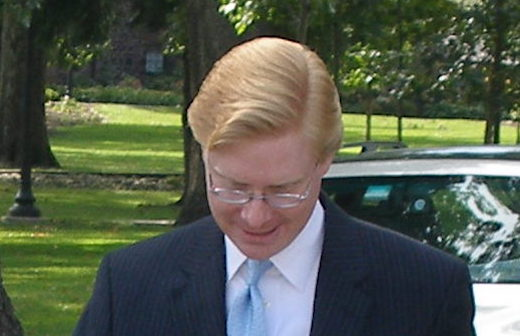
\includegraphics[width=.4\textwidth]{no_filter.jpg}
    \hspace{1mm}
    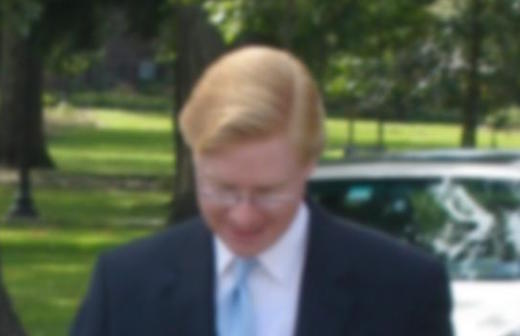
\includegraphics[width=.4\textwidth]{filter.jpg}
  \end{figure}
}
\end{frame}


\begin{frame}{Gradient Computation}
\tikzstyle{block_a} = [rectangle, draw, %fill=blue!20,
     text width=2em, text centered, rounded corners, minimum height=3em]
\tikzstyle{block_b} = [rectangle, draw, %fill=blue!20,
     text width=7em, text centered, rounded corners, minimum height=5em]
\tikzstyle{line} = [draw, -latex]


\footnotesize

\begin{tikzpicture}[node distance = 2.5cm, every text node part/.style={align=center}]
    % Place nodes
    \node [] (input_image) at (0,0) {$I(j,k)$};
    \node [] (node1) at (1.5,0) {};

    \node [block_a, above right of=node1,  node distance=2cm] (gradiente_x) {$h_x$};
    \node [] () at (5,1.65){$G_x(j,k)=I(j,k)*h_x$};

    \node [block_a, below right of=node1, node distance=2cm] (gradiente_y) {$h_y$};
    \node [] () at (4.75,-1.7){$G_y(j,k)=I(j,k)*h_y$};
    %\node [] (node2) at (4,0) {};
    \node [block_b] (combinazione) at (6,0) {$G=\sqrt{G_x^2+G_y^2}$ \\ $\theta=atan\left(\tfrac{G_y}{G_x}\right)$};
    \node[right of = combinazione](uscita){$\mathbf{G}(j,k)$};

    % Draw edges
    \path [draw, -] (input_image) -- (node1);
    \path [line] (node1) |- (gradiente_x);
    \path [line] (node1) |- (gradiente_y);
    \path [line] (gradiente_x) -| (combinazione);
    \path [line] (gradiente_y) -| (combinazione);
     %\path [line] (node2) -- (combinazione);
     \path [line] (combinazione) -- (uscita);
\end{tikzpicture}

\end{frame}


\begin{frame}{Histograms}

\only<1>{
  \begin{figure}[!ht]
  \centering
  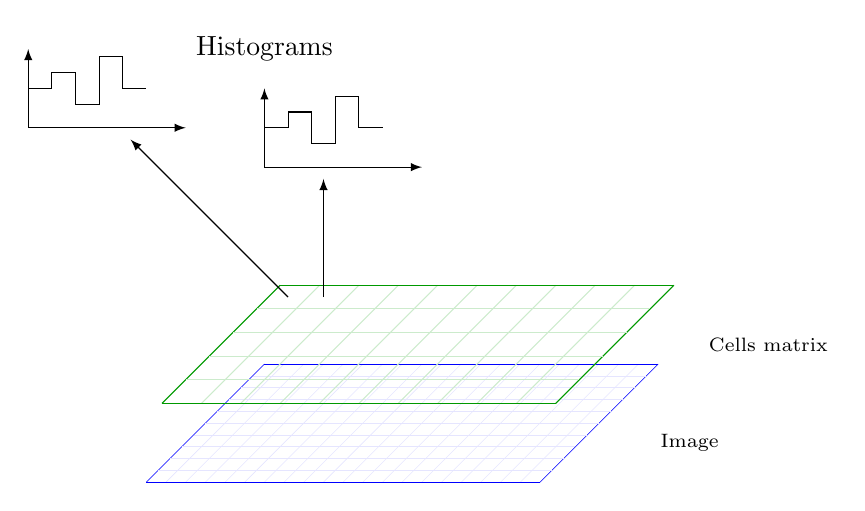
\begin{tikzpicture}[scale=1]

\foreach \x in {0,0.25,0.5,...,5} \draw[color=blue!10,very thin] (\x,0)--+(-1.5,-1.5);
\foreach \x in {0,5} \draw[color=blue,very thin] (\x,0)--+(-1.5,-1.5);

\foreach \y in {0,0.15,0.3,...,1.6 } \draw[color=blue!10,very thin] (-1*\y,-\y)--+(5,0);
\foreach \y in {0,1.5 } \draw[color=blue,very thin] (-1*\y,-\y)--+(5,0);

\node[] at (5.4,-1){{\scriptsize Image}};

\foreach \x in {0,0.5,1,...,5} \draw[color=green!60!black!20,thin] (\x+0.2,0+1)--+(-1.5,-1.5);
\foreach \x in {0,5} \draw[color=green!60!black,thin] (\x+0.2,0+1)--+(-1.5,-1.5);

\foreach \y in {0,0.3,0.6,...,1.6 } \draw[color=green!60!black!20,thin] (-1*\y+0.2,-\y+1)--+(5,0);
\foreach \y in {0,1.5 } \draw[color=green!60!black,thin] (-1*\y+0.2,-\y+1)--+(5,0);
\node[] at (6.4,0.25){{\scriptsize Cells matrix}};


\draw[-latex](0.3,0.85)--+(-2,2);
\draw[-latex](-3,3)--+(2,0);
\draw[-latex](-3,3)--+(0,1);
\draw[](-3,3.5)--+(0.3,0)--+(0.3,0.2)--+(0.6,0.2)--+(0.6,-.2)--+(0.9,-.2)--+(0.9,.4)--+(1.2,.4)--+(1.2,0)--+(1.5,0);

%
%
\draw[-latex](0.75,0.85)--+(0,1.5);
\draw[-latex](0.,2.5)--+(2,0);
  \draw[-latex](0.,2.5)--+(0,1);
  \draw[](0,3)--+(0.3,0)--+(0.3,0.2)--+(0.6,0.2)--+(0.6,-.2)--+(0.9,-.2)--+(0.9,.4)--+(1.2,.4)--+(1.2,0)--+(1.5,0);
  \node[] at (0,4){Histograms};
\end{tikzpicture}

  \caption{Spatial distribution of histograms and cells}
  \end{figure}
}

%------------------ SLIDE 2 ------------------
\only<2>{
  All the histograms are built as follows ($k=1,\ldots,n_\theta$):
  \begin{equation}
  H_c(k)=\sum_i\sum_jf[G(i,j)]\delta(\phi_{k-1}<\theta(i,j)<\phi_k)
  \end{equation}

  \begin{itemize}
  \item $n_\theta$ \emph{angle bins} uniformely (?) distributed
  \item The vote is a function of the gradient magnitude at the pixel $f(G)$, either the
        magnitude itself, its square, its square root, ...
  \end{itemize}
}
\end{frame}

\begin{frame}{Normalization}

\only<1>{
  \begin{figure}[!ht]
  \centering
  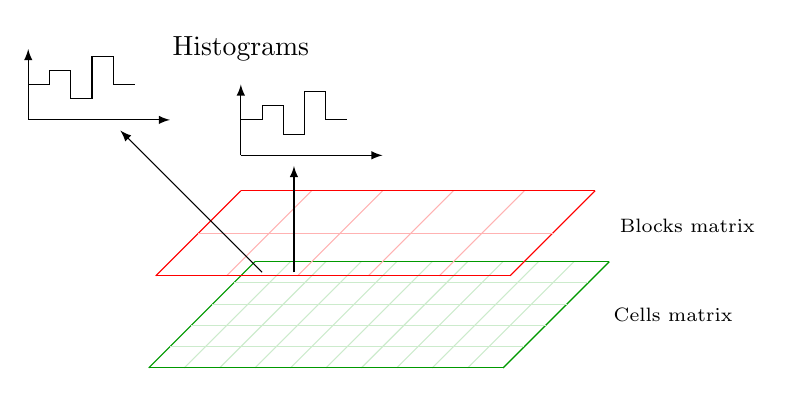
\begin{tikzpicture}[scale=0.9]
  
	\foreach \x in {0,0.5,1,...,5} \draw[color=green!60!black!20,thin] (\x+0.2,0+1)--+(-1.5,-1.5);
  \foreach \x in {0,5} \draw[color=green!60!black,thin] (\x+0.2,0+1)--+(-1.5,-1.5);

  \foreach \y in {0,0.3,0.6,...,1.6 } \draw[color=green!60!black!20,thin] (-1*\y+0.2,-\y+1)--+(5,0);
  \foreach \y in {0,1.5 } \draw[color=green!60!black,thin] (-1*\y+0.2,-\y+1)--+(5,0);
  \node[] at (6.1,0.25){{\scriptsize Cells matrix}};

	\foreach \x in {0,1,2,...,5} \draw[color=red!30,thin] (\x,0+2)--+(-1.2,-1.2);
  \foreach \x in {0,5} \draw[color=red,thin] (\x,0+2)--+(-1.2,-1.2);

  \foreach \y in {0,0.6,1.2 } \draw[color=red!30,thin] (-1*\y,-\y+2)--+(5,0);
  \foreach \y in {0,1.2 } \draw[color=red,thin] (-1*\y,-\y+2)--+(5,0);
  \node[] at (6.3,1.5){{\scriptsize Blocks matrix}};

	\draw[-latex](0.3,0.85)--+(-2,2);
	\draw[-latex](-3,3)--+(2,0);
	\draw[-latex](-3,3)--+(0,1);
	\draw[](-3,3.5)--+(0.3,0)--+(0.3,0.2)--+(0.6,0.2)--+(0.6,-.2)--+(0.9,-.2)--+(0.9,.4)--+(1.2,.4)--+(1.2,0)--+(1.5,0);

	\draw[-latex](0.75,0.85)--+(0,1.5);
	\draw[-latex](0.,2.5)--+(2,0);
  \draw[-latex](0.,2.5)--+(0,1);
  \draw[](0,3)--+(0.3,0)--+(0.3,0.2)--+(0.6,0.2)--+(0.6,-.2)--+(0.9,-.2)--+(0.9,.4)--+(1.2,.4)--+(1.2,0)--+(1.5,0);
  \node[] at (0,4){Histograms};

\end{tikzpicture}

  \caption{Spatial distribution of histograms, cells and blocks}
  \end{figure}
}

\only<2>{
  \small
  \metroset{block=fill}
  \begin{alertblock}{\textbf{Why?}}
  Gradient strengths vary over a wide range owing to local variations
  in illumination and foreground-background contrast, so effective local contrast
  normalization turns out to be essential for good performance.
  \end{alertblock}

  %\vspace{0.5cm}

  Possible normalization scheme:
  \begin{equation}
  H(c,k)= \frac{H_{1}(c,k)}{\left ( \sum_{c_i\in N_c} \sqrt{\|H_{1}(c_i)\|^2_2+\varepsilon^2}\right )}
  \end{equation}
  where $N_c$ is the set of all cells in a block.
}
\end{frame}

\begin{frame}{Results}

  \only<1>{
    \center
    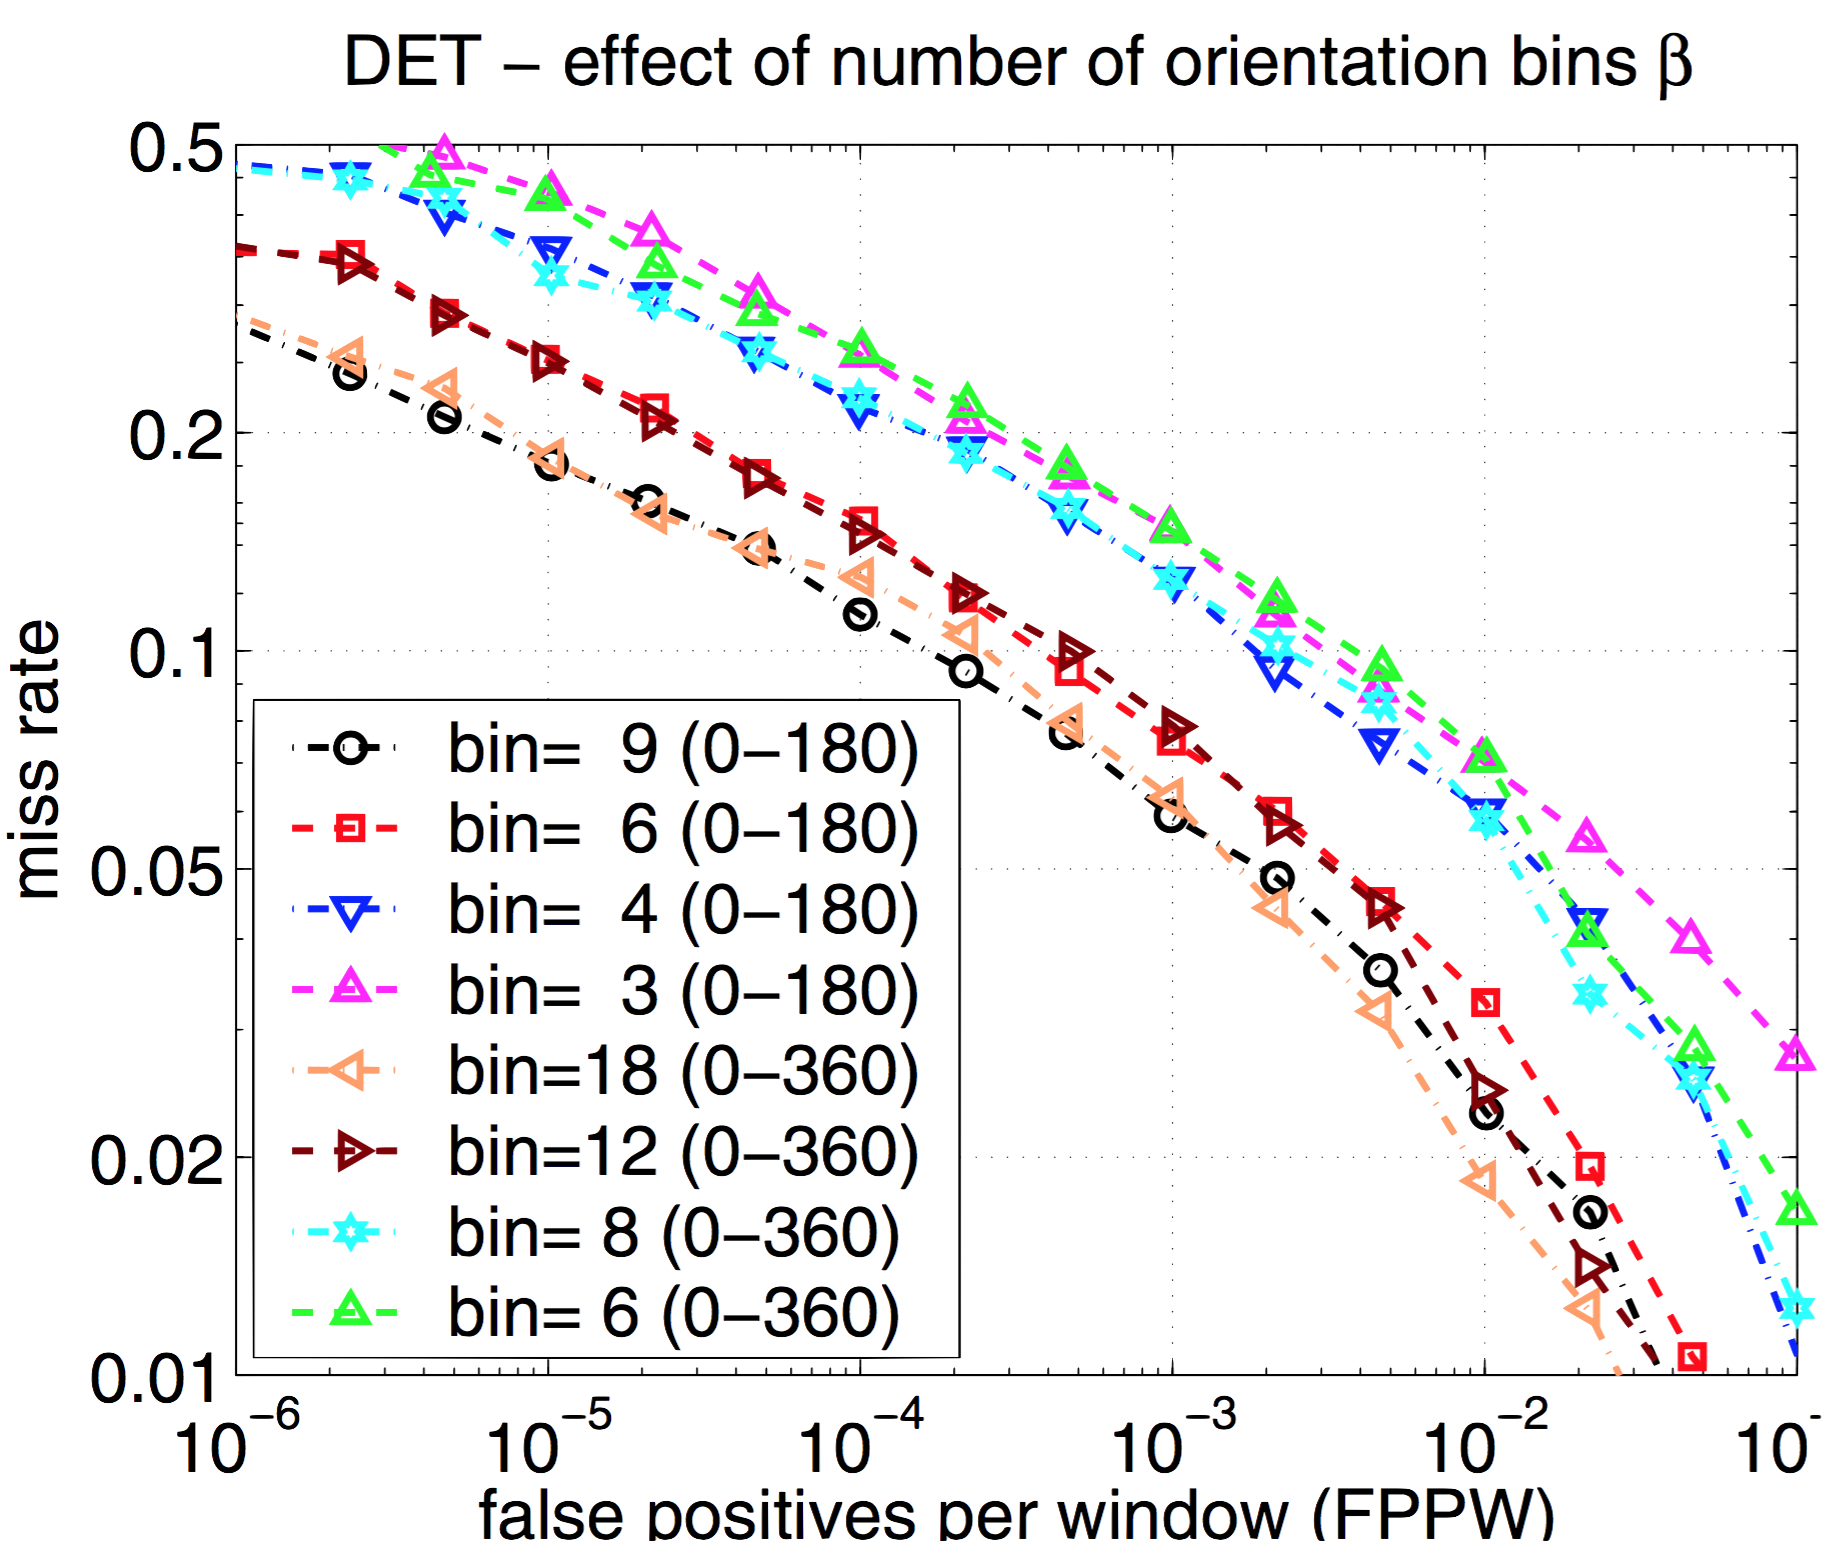
\includegraphics[width=0.75\textwidth]{HOG_result1.png}
  }

  \only<2>{
    \center
    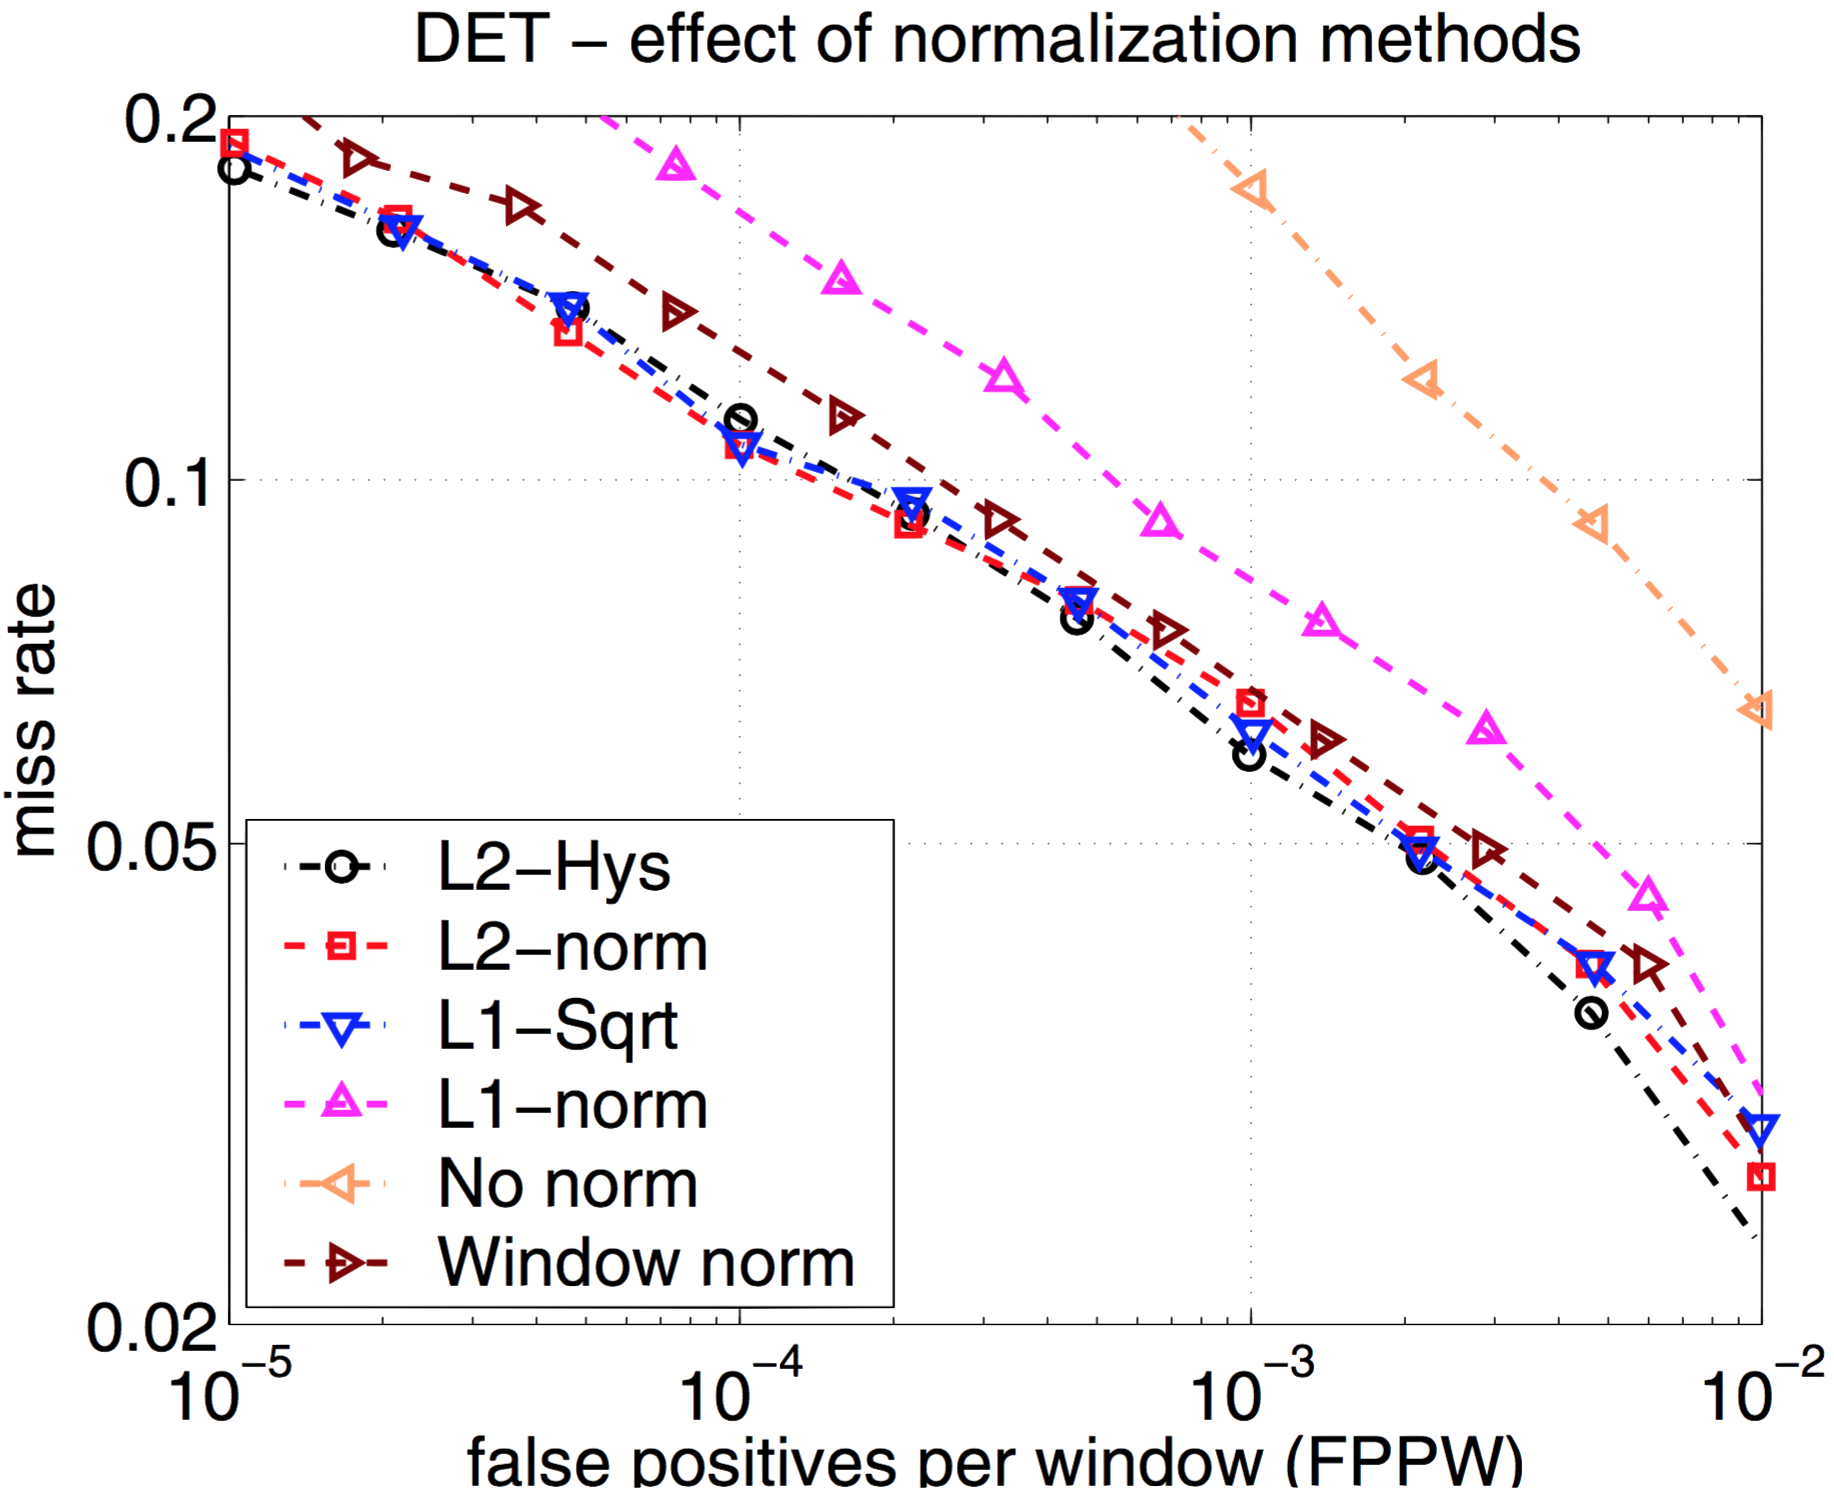
\includegraphics[width=0.75\textwidth]{HOG_result2.png}
  }

  \only<3>{
    \center
    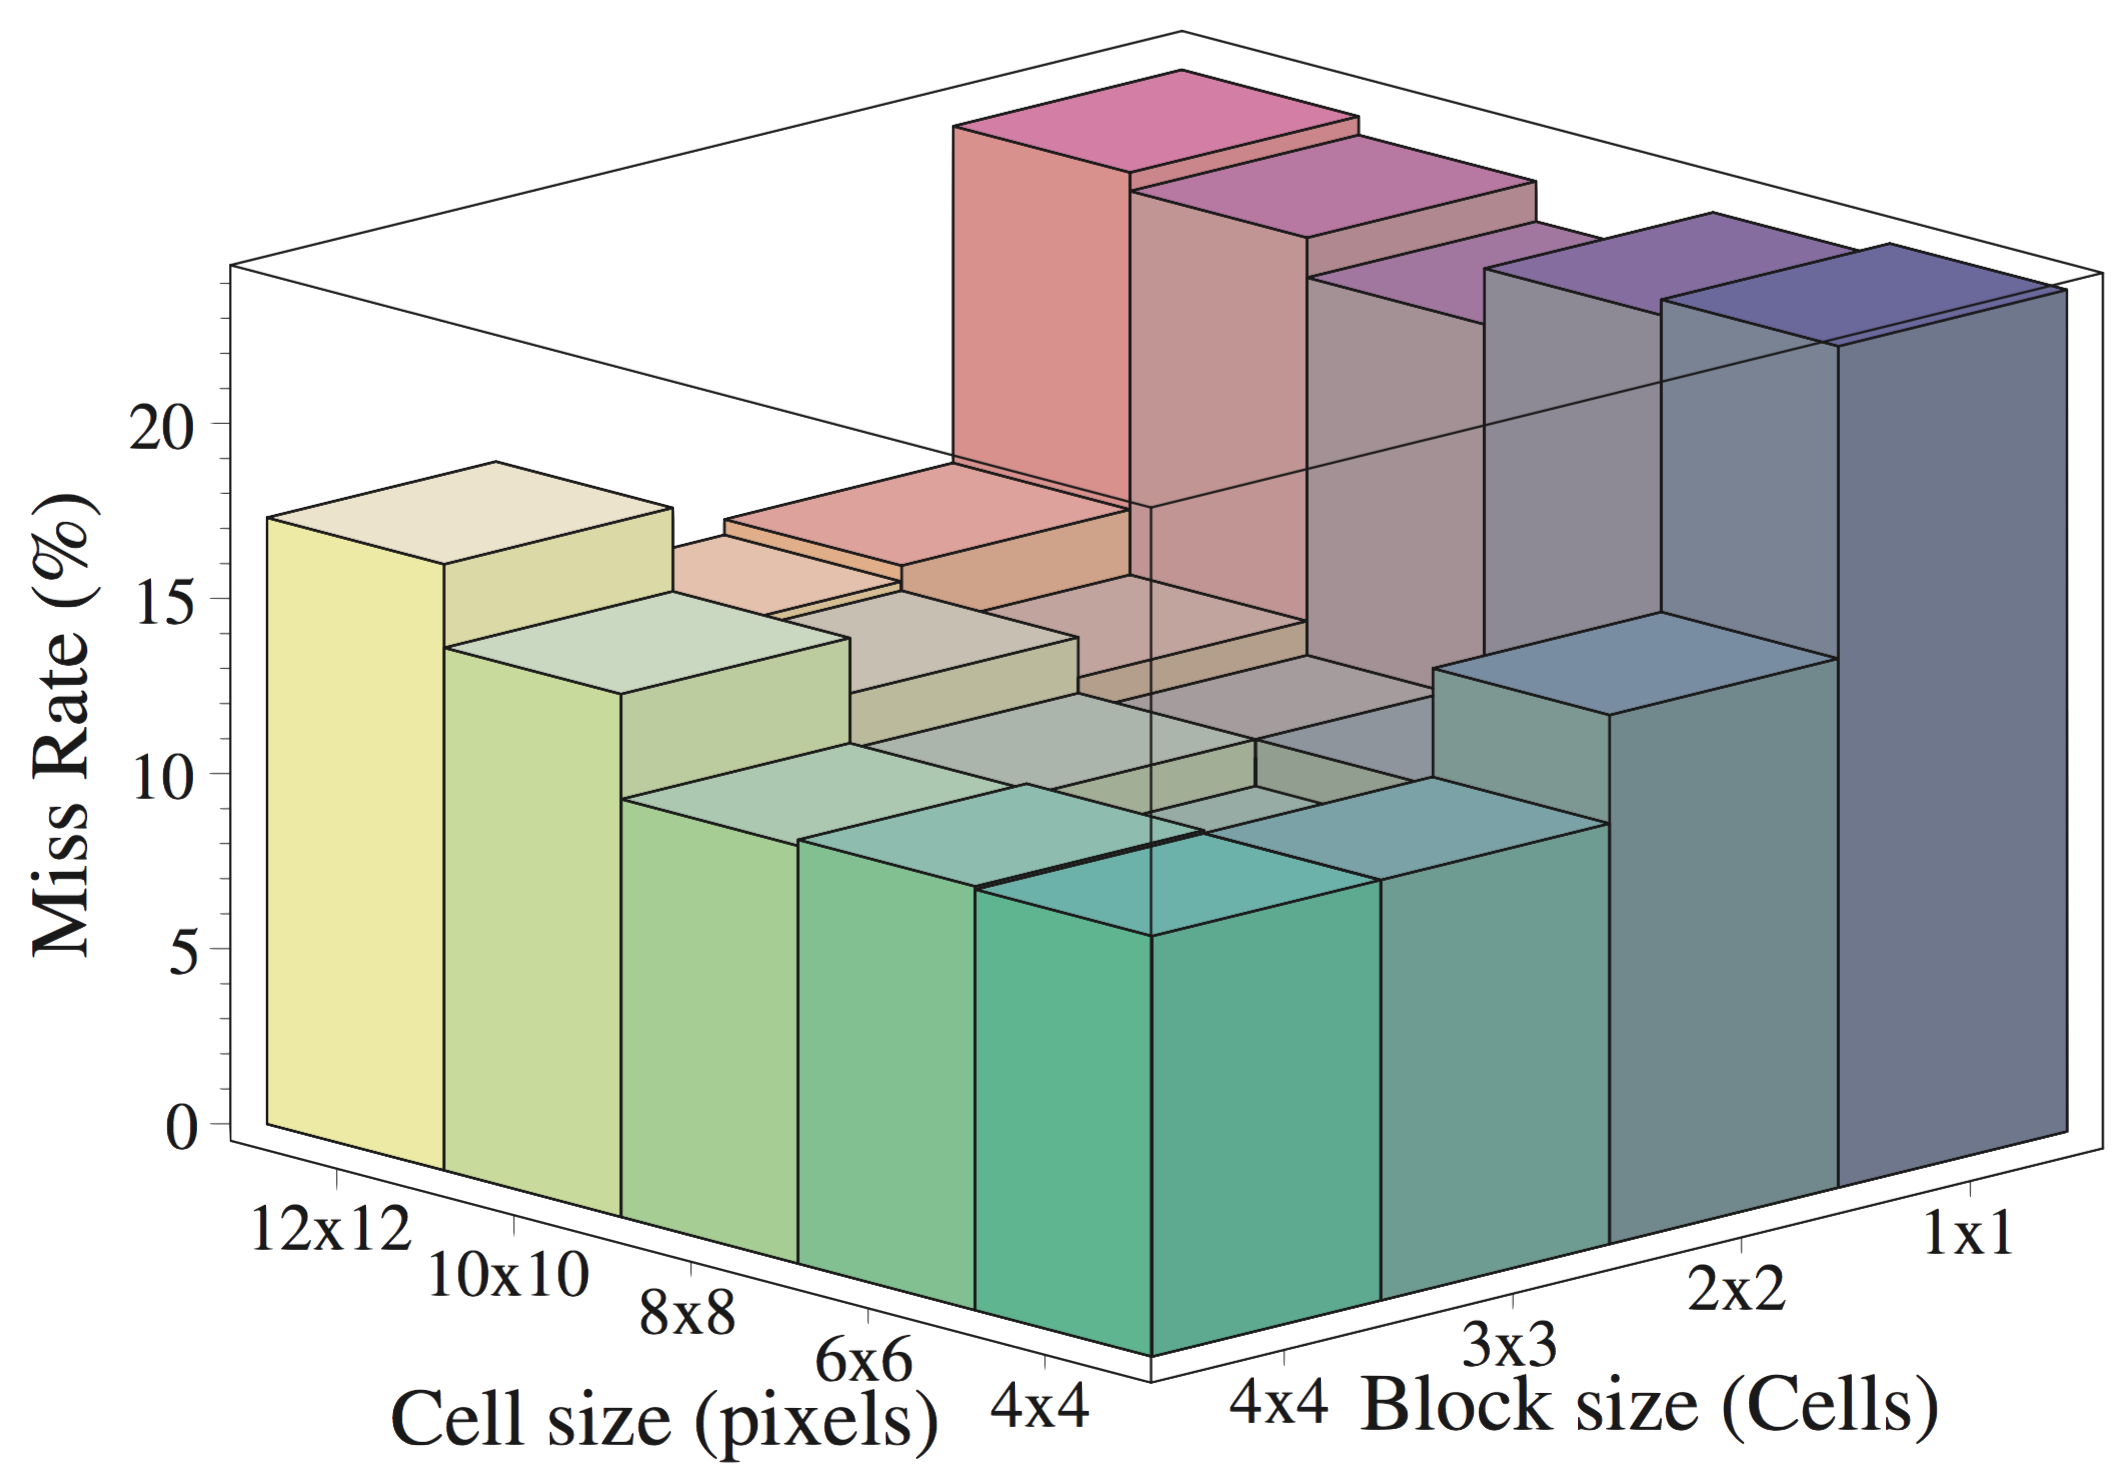
\includegraphics[width=0.75\textwidth]{HOG_result3.png}\\
    \small
    The miss rate at $10^{-4}$ FPPW as the cell and block sizes change.\\
    %3 x 3 blocks of 6 x 6 pixel cells perform best,
    %with 10.4\% miss rate.
  }

\end{frame}

\begin{frame}[standout]
  \huge Demo
\end{frame}

\begin{frame}{Demo}
  \centering
  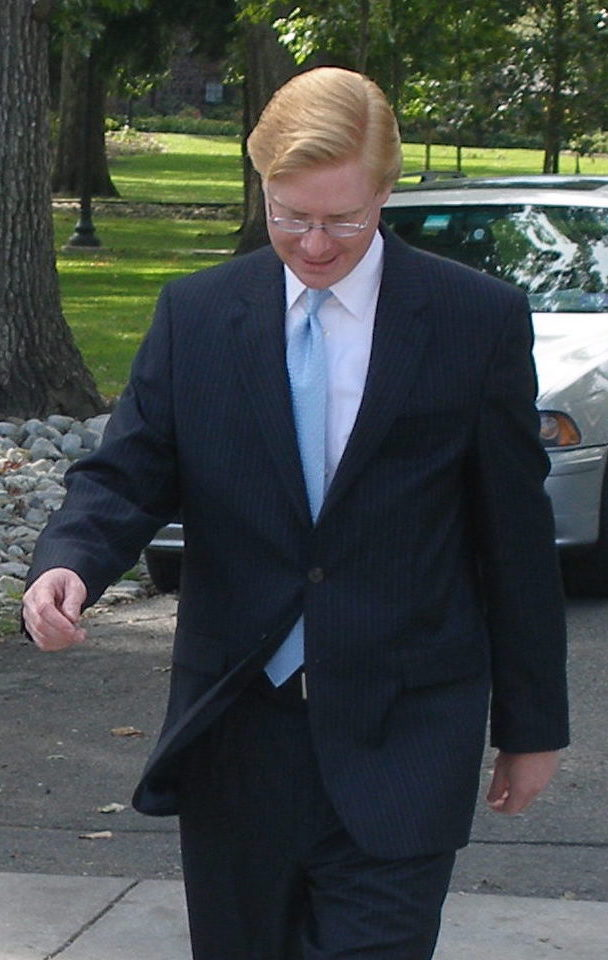
\includegraphics[height = .70\textwidth]{pedestrian.jpg}
  \hspace{2mm}
  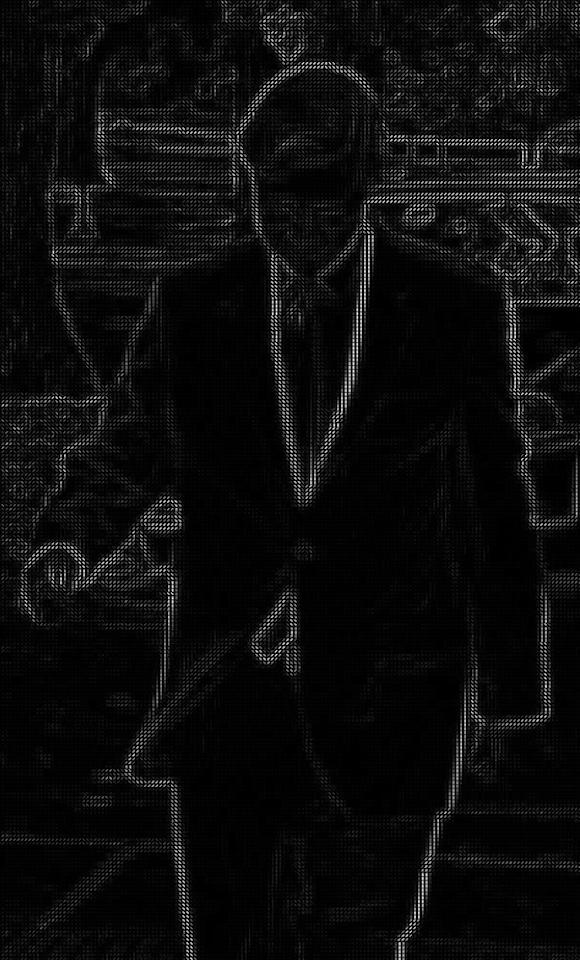
\includegraphics[height = .70\textwidth]{pedestrian_hog.jpeg}
\end{frame}

\begin{frame}{Summary}
  \small
  The HOG representation has several advantages. It captures gradient
  structure that is characteristic of local shape, with a representation invariant
  to local geometric and photometric transformations: translations or rotations make little difference
  if they are much smaller that the local spatial or orientation bin size. \\
  \vspace{5mm}
  For \textit{human detection}, \textbf{fine orientation sampling} and \textbf{strong
  local photometric normalization} turns out to be the best strategy: it permits body
  segments to change appearance and move from side to side quite a lot provided
  that they maintain an upright orientation.

\end{frame}
